\subsection{Evaluation of Energy Consumption, Wasted Traffic, and Connection Count}\label{sec:application:lte_video:numerical_evaluation}

In this section we study the metrics introduced in \refsec{sec:application:lte_video:system_model:model_assumptions:metrics} on the different transmission mechanisms.

First, we study the impact of the considered transmission mechanisms on the energy consumption and the wasted traffic. 
Then, we consider the impact of the connection count for the \streaming mechanisms and varying values of the parameters \emph{stop threshold} \bufferlower and \emph{threshold size} \buffersize in more detail.

We consider a video of \(\videolength=\SI{1600}{\second}\) length which is viewed on a \gls{UE} with \gls{LTE} access.
The median of available downlink throughput in current \gls{LTE} networks is \(\bandwidth = \SI{12.74}{\mega\bit\per\second}\) \cite{Huang2012}.
A wide set of video bit rates between \SIlist{1;50}{\mega\bit\per\second} is in use\footnote{\url{https://support.google.com/youtube/answer/1722171?hl=en}, \accessed}.
In order to prevent stalling, we consider bit rates between \SIrange{1}{10}{\mega\bit\per\second}, staying below the available network bandwidth.
For the \streaming mechanism, a stop threshold of \(\bufferlower = \SI{4}{\second}\) and a threshold size of \(\buffersize = \SI{32}{\second}\) were selected.
Furthermore, we specify a pre-buffering duration of \(\streamingstart = \SI{5}{\second}\).

We conduct our study using deterministic discrete event simulation which uses no random variables.
The wasted traffic is obtained analytically using the abort behaviour model.
Thus, all results are exact under the previously stated assumptions.

\subsubsection*{Energy Consumption}\label{sec:application:lte_video:numerical_evaluation:energy_consumption}
First, we study the influence of both video bit rate \bitrate as well as the selected download mechanism on energy consumption in \reffig{fig:application:lte_video:numerical_evaluation:energy_consumption:bitrate2energy}.
\begin{figure}
  \centering
  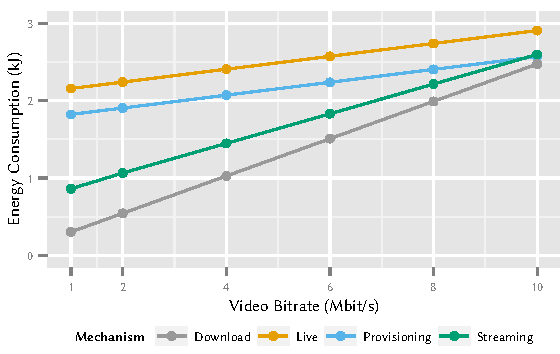
\includegraphics{application/lte_video/numerical_evaluation/figures/bitrate2energy}
  \caption{Influence of bit rate \bitrate and selected download mechanism on energy consumption \energyconsumption.}
  \label{fig:application:lte_video:numerical_evaluation:energy_consumption:bitrate2energy}
\end{figure}

We consider the \download mechanism and observe that it consumes the least amount of energy.
Here the video is downloaded with full bandwidth, as seen in \reffig{fig:application:lte_video:system_model:video_model}, resulting in a very short energy intensive download phase and a longer energy playback phase which consumes less energy.
For the \live mechanism we observe the opposite, i.e. the highest energy consumption for all bandwidths.
If this mechanism is used, the used bandwidth equals the video bit rate \bitrate.
Thus, the download requires the same amount of time as the playback, resulting in the highest possible energy consumption \energyconsumption.
The \serviceprovisioning method uses a higher bandwidth, thus reducing the overall download time.
This reduced download time decreases the energy consumption \energyconsumption when compared to the \live mechanism, even though the bandwidth used for downloading is increased to \SI{120}{\percent}.
For the \streaming mechanism we observe an energy consumption \energyconsumption slightly higher than the \download mechanism.
As the bit rate \bitrate of the video increases, the energy consumption \energyconsumption increases as well.
This is due to the fact that a higher video bit rates \bitrate require larger downloads.
For video bit rates \bitrate approaching the available bandwidth the \streaming mechanism degenerates to the \live mechanism, as no pre-buffering is possible.
We conclude that the \download and \streaming mechanisms outperform \live and \serviceprovisioning with regard to energy consumption.

\subsubsection*{Wasted Traffic}\label{sec:application:lte_video:numerical_evaluation:wasted_traffic}
Next, we consider the wasted traffic \meanwastedtraffic as a metric of the transmission mechanism quality.
If a user completely watches a video, no traffic is wasted, as all data downloaded is used during playback.
Thus, we consider only the cases where a user stops the playback before the video is finished.

\begin{figure}
  \centering
  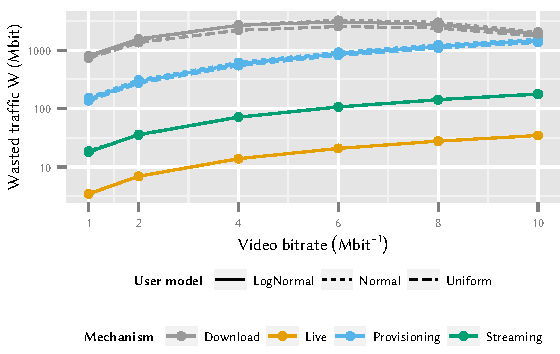
\includegraphics{application/lte_video/numerical_evaluation/figures/bitrate2lostData}
  \caption{Influence of bit rate \bitrate, download mechanism and user model on the mean wasted traffic \meanwastedtraffic. Download, Live, and Provisioning mechanisms result in equal connection counts.}
  \label{fig:application:lte_video:numerical_evaluation:energy_consumption:bitrate2lostData}
\end{figure}

In \reffig{fig:application:lte_video:numerical_evaluation:energy_consumption:bitrate2lostData} we study the mean wasted traffic \meanwastedtraffic for different video bit rates \bitrate.
We consider the different transmission mechanisms introduced in \refsec{fig:application:lte_video:system_model:video_model} as well as the previously introduced user models.
We observe that the choice of user model has no significant impact on the mean wasted traffic \meanwastedtraffic.
For the \download mechanism, the amount of mean wasted traffic \meanwastedtraffic increases up to a video bit rate \bitrate of \SI{6}{\mega\bit\per\second}, then the mean wasted traffic \meanwastedtraffic decreases as only video data which has been pre-buffered can be lost if the user aborts the video.
As we assume an available bandwidth of \SI{12.74}{\mega\bit\per\second}, the bandwidth available for pre-buffering decreases as the bit rate \bitrate increases, resulting in lower amounts of mean wasted traffic \meanwastedtraffic for high video bit rates \bitrate.
For the \live mechanism, we see that the wasted traffic for all user models is very low, but wasted traffic exists.
This is due to the traffic already sent by the server while the \gls{UE} is still waiting for promotion from \rrcidle to \rrcconnected, i.e. a short pre-buffering phase exists.
As the bandwidth increases with the video bit rate \bitrate, the mean wasted traffic \meanwastedtraffic increases as well.
Next, we consider the \serviceprovisioning approach and see an increase of mean wasted traffic \meanwastedtraffic as the video bit rate \bitrate increases, due to the fact that the bandwidth used for continuous download is a factor of the video bit rate \bitrate.
A higher video bit rate \bitrate results in the download of the video being completed earlier, which leads to more mean wasted traffic \meanwastedtraffic.
Similar results can be seen for the \streaming mechanism, which results in more mean wasted traffic \meanwastedtraffic than the \live mechanism, but significantly less traffic than the \serviceprovisioning mechanism.
This is due to the fact that if the user aborts, at least the amount of video given by the \emph{stop threshold} \bufferlower and at most the complete buffer, given by the \emph{stop threshold} and the \emph{threshold size} are lost.
We have observed that the choice of user model results in no qualitative changes in mean wasted traffic \meanwastedtraffic.
As described in the last paragraph, the \download and \streaming mechanisms provide best results with regard to energy consumption.
However with regard to wasted traffic, the \live and \streaming mechanisms are most suited.
Thus, the \streaming mechanism seems to be a good compromise.
The network operator can select a tradeoff between energy consumption and mean wasted traffic \meanwastedtraffic as discussed in the next section.
From now on, we only consider the uniformly distributed user model.

\subsubsection*{Connection Count}\label{sec:application:lte_video:connection_count}
The \gls{ISP} is interested in reducing the number of connections occurring during video transmission.
Thus, we quantify the impact of the selected video transmission mechanism on the connection count \connectioncount, which directly correlates with the occurring signalling.

\begin{figure}
  \centering
  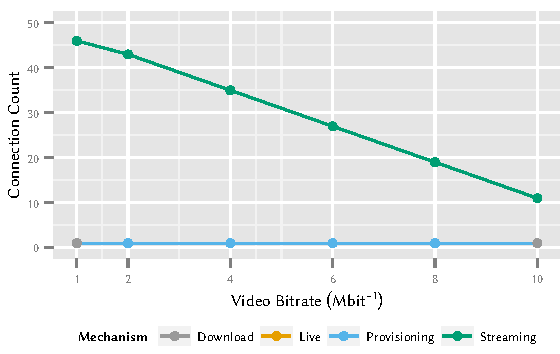
\includegraphics{application/lte_video/numerical_evaluation/figures/bitrate2connections}
  \caption{Influence of bit rate \bitrate and selected download mechanism on the connection count \connectioncount.}
  \label{fig:application:lte_video:numerical_evaluation:energy_consumption:bitrate2connections}
\end{figure}

In \reffig{fig:application:lte_video:numerical_evaluation:energy_consumption:bitrate2connections} we study the impact of the different transmission mechanisms on the number of connections per transmission and thus the amount of generated signalling.
We observe that for the transmission mechanisms download, live, provisioning the connection count \connectioncount is constantly one, independent of the selected bit rate \bitrate.
This is due to the fact that in these transmission mechanisms the video is transmitted in one chunk.
For streaming, the connection count \connectioncount decreases as the video bit rate \bitrate increases.
Here, a connection occurs each time the buffer is refilled.
For larger bit rates \bitrate, refilling the buffer requires a longer transmission.
As the maximum time of video transmission is upper bounded by the video length, longer buffering phases result in a smaller total amount of buffering phases and thus in a smaller connection count \connectioncount per video transmission.

\begin{figure}
  \centering
  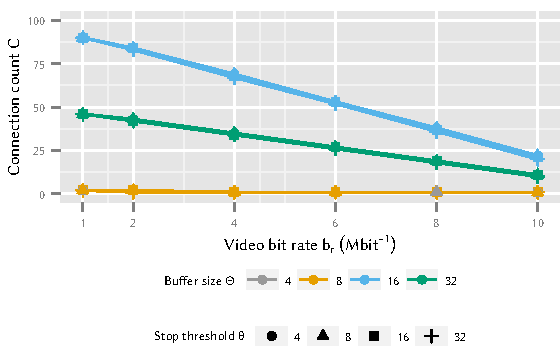
\includegraphics{application/lte_video/numerical_evaluation/figures/bitrate2connections_parameters}
  \caption{Influence of bit rate \bitrate and selected parameters on the connection count \connectioncount for the streaming mechanism. Lines for different stop thresholds \(\theta\) overlap.}
  \label{fig:application:lte_video:numerical_evaluation:energy_consumption:bitrate2connections_parameters}
\end{figure}

Next, we consider the impact of the stop threshold~\bufferlower and buffer size~\buffersize on the connection count \connectioncount caused by the \streaming mechanism.
In \reffig{fig:application:lte_video:numerical_evaluation:energy_consumption:bitrate2connections_parameters} we observe that while the buffer size has a significant impact on the connection count \connectioncount during a video transmission, the lower buffer threshold has almost no impact.
For buffer sizes of \SIrange{4}{8}{\second}, no new connections are started, i.e. no signalling occurs.
This is due to the fact that the connection timeout in \gls{UE} is configured as \SI{11.576}{\second}, as discussed in \refsec{sec:application:lte_video:system_model:lte_network_model}.
Thus, for this low buffer sizes the \gls{UE} does not disconnect from the network.
Furthermore, we observe that as the buffer size increases, the number connection count \connectioncount decreases.
Refilling larger buffers requires, similar to larger bit rates \bitrate, longer transmission times.
Thus, due to the total upper bound on the transmission time, less download phases can occur during the transmission.